%HEURISTIC TREES IN COMPLEX FORESTS
%COPYRIGHT@SCHULZ, SPEEKENBRINK & MEDER

\documentclass[a4paper,man, natbib]{apa6}
\usepackage[english]{babel}
\usepackage[utf8x]{inputenc}
\usepackage{bbm}
\usepackage{amsmath}
\usepackage{graphicx}
\usepackage[colorinlistoftodos]{todonotes}
\usepackage{geometry}
\usepackage{natbib}
\usepackage{epsfig}
\usepackage{upgreek}
\usepackage{bbold}
\usepackage{setspace}
\usepackage{caption}
\usepackage{float}
\usepackage{placeins}
\usepackage{tikz}
\usetikzlibrary{positioning,shadows,arrows}
\usepackage{natbib}
\usepackage{amsmath,amsfonts,amsthm,amssymb}
\usepackage{url}
\usepackage{multirow}
\usepackage{subfigure}
\usepackage{algorithm}
\usepackage[noend]{algpseudocode}


%%%%%%%%%%%%%%%%%%%%%%%%%%%%%%%%%%%%%%%%%%%%%%%%%%%%%%%%%%%%%%%%%%%%%%%%%%%%%%%%%%%%%%%%%%%%%%%%%%%
%TITLE PAGE
%%%%%%%%%%%%%%%%%%%%%%%%%%%%%%%%%%%%%%%%%%%%%%%%%%%%%%%%%%%%%%%%%%%%%%%%%%%%%%%%%%%%%%%%%%%%%%%%%%%
\title{Simple Trees in Complex Forests: Growing Heuristics through Approximate Bayesian Computation}
\shorttitle{Simple Trees in Complex Forests}
\threeauthors{Eric Schulz}{Maarten Speekenbrink}{Bj\"orn Meder}
\threeaffiliations{Department of Experimental Psychology\\University College London}{Department of Experimental Psychology\\University College London}{Center for Adaptive Behavior and Cognition\\ Max Planck Institute for Human Development, Berlin}

%%%%%%%%%%%%%%%%%%%%%%%%%%%%%%%%%%%%%%%%%%%%%%%%%%%%%%%%%%%%%%%%%%%%%%%%%%%%%%%%%%%%%%%%%%%%%%%%%%%
%ABSTRACT
%%%%%%%%%%%%%%%%%%%%%%%%%%%%%%%%%%%%%%%%%%%%%%%%%%%%%%%%%%%%%%%%%%%%%%%%%%%%%%%%%%%%%%%%%%%%%%%%%%%
\abstract{Heuristic models of decision making have historically been unable to explain how elaborate heuristic strategies can emerge from smaller building blocks. We propose Approximately Bayesian Computed Take-The-Best (TTB-ABC) as a solution to this problem. Using this algorithm, we show how non-compensatory strategies such as Take-The-Best can emerge from smaller probabilistically updated building blocks without relying on heavy computation. Based on a self-reinforcing sampling scheme, different non-compensatory building blocks are proposed and, over time, tree-like heuristics emerge. We demonstrate that TTB-ABC is able to recover a data set that was generated by standard Take-The-Best, leads to sensible inferences about cue validities, can outperform Take-The-Best, and trades-off performance and computational complexity explicitly. This constitutes as a first proof of concept of how a tool from the heuristic tool box can emerge from smaller building blocks.}

\begin{document}
\maketitle

%%%%%%%%%%%%%%%%%%%%%%%%%%%%%%%%%%%%%%%%%%%%%%%%%%%%%%%%%%%%%%%%%%%%%%%%%%%%%%%%%%%%%%%%%%%%%%%%%%%
%INTRODUCTION
%%%%%%%%%%%%%%%%%%%%%%%%%%%%%%%%%%%%%%%%%%%%%%%%%%%%%%%%%%%%%%%%%%%%%%%%%%%%%%%%%%%%%%%%%%%%%%%%%%%
\section{Introduction}
A main problem within the literature of heuristic decision making can be called the \emph{strategy emergence problem} and it reads as follows: How can a heuristic strategy evolve from smaller building blocks over time? Take the heuristic \emph{Take-The-Best} (henceforth TTB) as an example \citep{gigerenzer1999betting}: TTB is a non-compensatory strategy to choose between two options \citep{hoffrage1999people}. Non-compensatory means that, if one orders the used variables in terms of their importance, the first variable has a stronger effect than all the other variables combined, the second variable has a stronger effect than all the remaining variables combined, and so forth. In fact, it is postulated that once a variable is able to decide between the options, the other variables are not even looked up any further. Consider the decision about which of two cities has a larger population size and let us assume that the two compared cities can be described by answering the following yes-no-questions:
\begin{description}
		\item[$\mathcal{Q}1$:]Is it a capital city?
		\item[$\mathcal{Q}2$:] Does it have an airport?
		\item[$\mathcal{Q}3$:] Does it have a major league football team?
		\item[$\mathcal{Q}4$:] Is it a trade fair town?
\end{description}
In order to compare two cities, one only has to look up the questions Q1-Q4 in the above order. As soon as one criterion weighs favorably for one city over the other, the comparison stops and the response is that the city with the favorable cue is bigger. For example, comparing London and Manchester, one could ask ``Is one of them a capital city?'', which is true for London, but false for Manchester and at which point the comparison stops and the final response is to say that London is bigger. Comparing Manchester and Oxford, one would ask Q1, which is false for both; then Q2, true for both; and then Q3, which is only true for Manchester. Thus, the final response is to say that Manchester is bigger than Oxford. If none of the questions can distinguish between the options, for example, comparing London and Paris, then the final remedy would be to guess. Although relatively simple, TTB has been shown to perform surprisingly well in many different classification tasks such as predicting city sizes, professors' salaries, high school drop out rates, and homelessness of US-American cities \citep{gigerenzer1999simple}, to name but a few. Yet, TTB also provides an almost paradigmatic example of the \emph{strategy emergence problem}: this problem arises when taking the adaptive toolbox metaphor literally \citep{gigerenzer2011heuristic}. The adaptive toolbox is normally assumed to contain different building blocks that loosely fall within 3 categories: \emph{Search rules} dictate how a decision maker looks up information, for example sequentially from Q1 to Q4. \emph{Stopping rules} tell us when to stop the search, for example as soon as one of the 4 question is answered with a yes for one but not for the other city. Lastly, \emph{decision rules} make the actual decision after the search has been stopped, for example, indicating that the city with a major football league team is bigger than the city without one. If we now look at these three rules, we see that all of the building blocks, that is the search, the stopping, and the decision rule are already given. The only thing a decision maker has to learn over time is the question order, also sometimes referred to as cue validity. Commonly, TTB's cue validity is determine by how well the different questions can predict the observed outcome \citep{broder2000assessing}. This definition, however, completely ignores the question of how a decision maker knows that she can apply exactly these three rules in a given scenario. Contrarily, in keeping with the original definition of the heuristic toolbox, one would assume that a decision maker approaches a problem with a set of search, stopping, and decision rules in mind and --over time-- learns how to combine these rules successfully. This combination, in the end, might result in a non-compensatory model that looks like TTB. Even more, one would assume that there exist smaller rules that together compose increasingly bigger heuristics such as how to choose a particular strategy. Therefore, we think that a viable theory of heuristic decision making has to explain the dynamics of the heuristic toolbox; it has to explain how different building blocks are combined and heuristic strategies emerge. However, none of the current approaches towards heuristic decision making addresses this problem explicitly . It is this explanatory dearth that motivates this paper.

In what follows, we will introduce and define TTB-ABC (Approximately Bayesian Computed Take-The-Best), a novel algorithm that can learn non-compensatory decision strategies on the fly by using approximate Bayesian computation of sampled building blocks. This approach does not need complicated likelihood manipulations, but rather depends on the acceptance and rejection of simple mental simulations. When heuristic subunits are fed into this algorithm, a powerful yet elegant machinery is created that learns non-compensatory strategies by mimicking a Bayesian reinforcement learning algorithm. It will be shown that this approach can recover structures that are solely based on traditional TTB, leads to sensible inferences about cue validities, outperforms traditional TTB-models, and can be utilized to trade-off performance and computational complexity explicitly. To the best of our knowledge, this provides a first ever proof of concept of how a heuristic can emerge from smaller building blocks.


%%%%%%%%%%%%%%%%%%%%%%%%%%%%%%%%%%%%%%%%%%%%%%%%%%%%%%%%%%%%%%%%%%%%%%%%%%%%%%%%%%%%%%%%%%%%%%%%%%%
%EXPLAINING ABC + EXAMPLE
%%%%%%%%%%%%%%%%%%%%%%%%%%%%%%%%%%%%%%%%%%%%%%%%%%%%%%%%%%%%%%%%%%%%%%%%%%%%%%%%%%%%%%%%%%%%%%%%%%%
\section{Approximate Bayesian Computation}
The goal of Bayesian inference is to calculate the posterior of a parameter $\theta$, given some prior $\pi(\theta)$ and having observed some data $\mathcal{D}$ \citep{lindley1972bayesian}.

%Bayesian Posterior Calculation
\begin{align}
p(\theta|\mathcal{D})&=\frac{p(\mathcal{D}|\theta)\pi(\theta)}{\int_{\theta} p(\mathcal{D}|\theta)\pi(\theta) \text{d} \theta}\\
& \propto p(\mathcal{D}|\theta)\pi(\theta)
\end{align}
%End of Bayesian Posterior Calculation

This means that the posterior depends on the prior belief $\pi(\theta)$ about $\theta$ via the likelihood of the observed data $p(\mathcal{D}|\theta)$ under that particular prior. Bayesian inference can provide a strong tool to cope with uncertainty as it models a person's subjective beliefs of the world as a mixture of prior assumptions and incoming data. It is therefore not surprising that it has been used to model cognition in many different domains \citep{oaksford2007bayesian}. However, Bayesian inference also suffers from potentially high computational costs and, occasionally, from analytical intractability \citep{dagum1993approximating}. For many of those problems, sophisticated sampling schemes have been developed that approximate the posterior distribution by the means of Monte Carlo Markov chains \citep{gilks2005markov}. This and an increase in computational power has lead to what has been referred to as the ``Bayesian Revolution'', the increased application of of Bayesian models, over the last decades \citep{brooks2003bayesian}. It has even be claimed that some classic psychological effects such as anchoring or the availability bias can be explained by sampling-based models similar to MCMC \citep{lieder2012burn}. Here, we want to focus on a strategy that sounds simple at first, but turns out to be an elegant approach to approximate posterior inference. This strategy is called \emph{Approximate Bayesian Computation} \citep{turner2012tutorial}. Approximate Bayesian Computation (ABC) is an approximative method that, instead of computing the required likelihood directly, substitutes it with surrogate simulations of a given model \citep{csillery2010approximate}.

%This is the lamest example ever. Would appreciate if you can come up with something better...
Imagine that you are trying to figure out how much water you should use to water a plant. You have some expectations about how different amounts of water might lead to different growth rates. Additionally, you might have some priors about what a sensible amount of water might be; 0.01 litre probably will not help your plant to grow a lot. What Approximate Bayesian Computation now means is that you observe different growth rates in the world and that you internally simulate realizations of your priors when plugged into your model (your explanation of the world) and only keep the ones that come out reasonably close to what you have actually observed. This simple mechanism of internalized mental simulations and external reality checks provides a useful tool to approximate posteriors. A more formal description of ABC is shown in Algorithm~\ref{alg:abc}.
 
%BEGIN OF ABC ALGORITHM
\FloatBarrier
\begin{algorithm}
\caption{Approximate Bayesian Computation}
\label{alg:abc}
\input{algs/abc.alg}
\end{algorithm}
\FloatBarrier
%END OF ABC ALGORITHM

This algorithm samples a proposed parameter from a prior $\pi(\theta)$ and plugs the proposal into a model $\mathcal{M}$ in order to simulate an output $\mathbf{y^*}$ from the given data $\mathcal{D}$ at hand. It then calculates a summary statistic $\mathcal{S}$ of both the simulated data and the real data and accepts proposals that have produced a summary that is reasonably close to the summary of the real data, allowing for some error $\epsilon$. The proximity of the two summary statistics is normally estimated by a measure of distance $\delta$, for example the euclidean distance. A more psychological explanation of this algorithm is that an agent has some prior assumptions about how the world works and repeatedly checks whether or not these prior assumptions can, on average, produce similar patterns to the ones seen by applying constant mental simulations; that is sanity-checking if the assumption are good enough to produce the seen outcomes. If they are, then those assumptions are accepted. If they are not, then they are rejected. Even though this algorithm sounds simple, it has been shown to approximate posteriors well for many complex scenarios and is currently the topic of vivid ongoing research debates. In particular, ABC has been described to be ``embarrassingly parallelizable'' as the aforementioned simulation-based approach can easily be set up on many different computing units \citep{marjoram2003markov} and can be used in scenarios where the likelihood is intractable.

For a simple example, consider the case of a linear regression with only one parameter as shown in Equation~\ref{eq:regexample}.

%LINEAR REGRESSION EXAMPLE
\begin{align}
\label{eq:regexample}
y&=\beta x +\epsilon\\
\epsilon &\sim \mathcal{N}(0,\sigma^2)
\end{align}
%END OF LINEAR REGRESSION EXAMPLE

Of course, one could simply use standard Bayesian calculations to estimate the posterior of $\beta$. However, here we want to demonstrate how ABC can be used to approximate a posterior distribution when we know the underlying truth. For this simple example, 1000 observations of a single variable $\mathbf{x}$ were created to be distributed normally $\mathbf{x}\sim\mathcal{N}(0,0.1)$, $\beta$ was fixed to be $1$, and the dependent variable $\mathbf{y}$ was simulated as in Equation~\ref{reg1}. ABC then was implemented based on a uniform prior $\pi(\beta)\sim\mathcal{U}[-5,5]$ and 100,000 simulations were created from that prior. These simulations were then used to create a proposed output vector $\mathbf{y_{\text{prop}}}$. Afterwards, the Euclidean distance (see Equation~\ref{eq:eucliddist}) between the generated and the observed data, based on 100 sampled data points, was calculated and tracked for every proposed sample.

%EUCLIDEAN DISTANCE
\begin{align}
\label{eq:eucliddist}
\rho(\mathbf{x},\mathbf{y})=\frac{1}{n}\sum_{i=1}^{n}\sqrt{(x_i-y_i)^2}
\end{align}
%END OF EUCLIDEAN DISTANCE

This situation can be easily described as before: if we want to find out how much water leads to different rates of plant growth, then we could check different data pairs of water and growths from the past, mentally simulate outcomes, and check if the simulated growth is somewhat similar to the observed growth.
Figure~\ref{fig:linexample} shows the true underlying data, the simulation results of the distances as well as the posterior estimate of $\beta$ depending on different values of $\epsilon$. The true underlying data is just based on the model defined above. The produced distances based on 100,000 simulation from the prior demonstrated that many proposal ended up close to a distance of 0. This is due to the fact that we had a good prior assumption about $\beta$. The last graph shows different posterior estimates for $\beta$ depending on how low $\epsilon$ was set. We can also see that the posterior estimates become more exact, the lower we set $\epsilon$. Indeed, if $\epsilon$ was set to 0, we would get pure rejection sampling. If we had set it to infinity, then ABC would have returned the prior as posterior as all proposals would have been accepted. Finally, the standard error for our posterior estimates gets slightly bigger, the lower we set $\epsilon$. This is due to the fact that more samples will be deemed useless and therefore thrown away for low $\epsilon$s:  we notice that ABC can be wasteful, especially when the prior is far away from the true posterior. 

%PLOT OF ABC EXAMPLE OUTCOMES
\begin{figure}[htb!]
  \caption{Plots of underlying data, the resulting distances, and the posterior mean dependent on $\epsilon$.}
\label{fig:linexample}
  \centering
    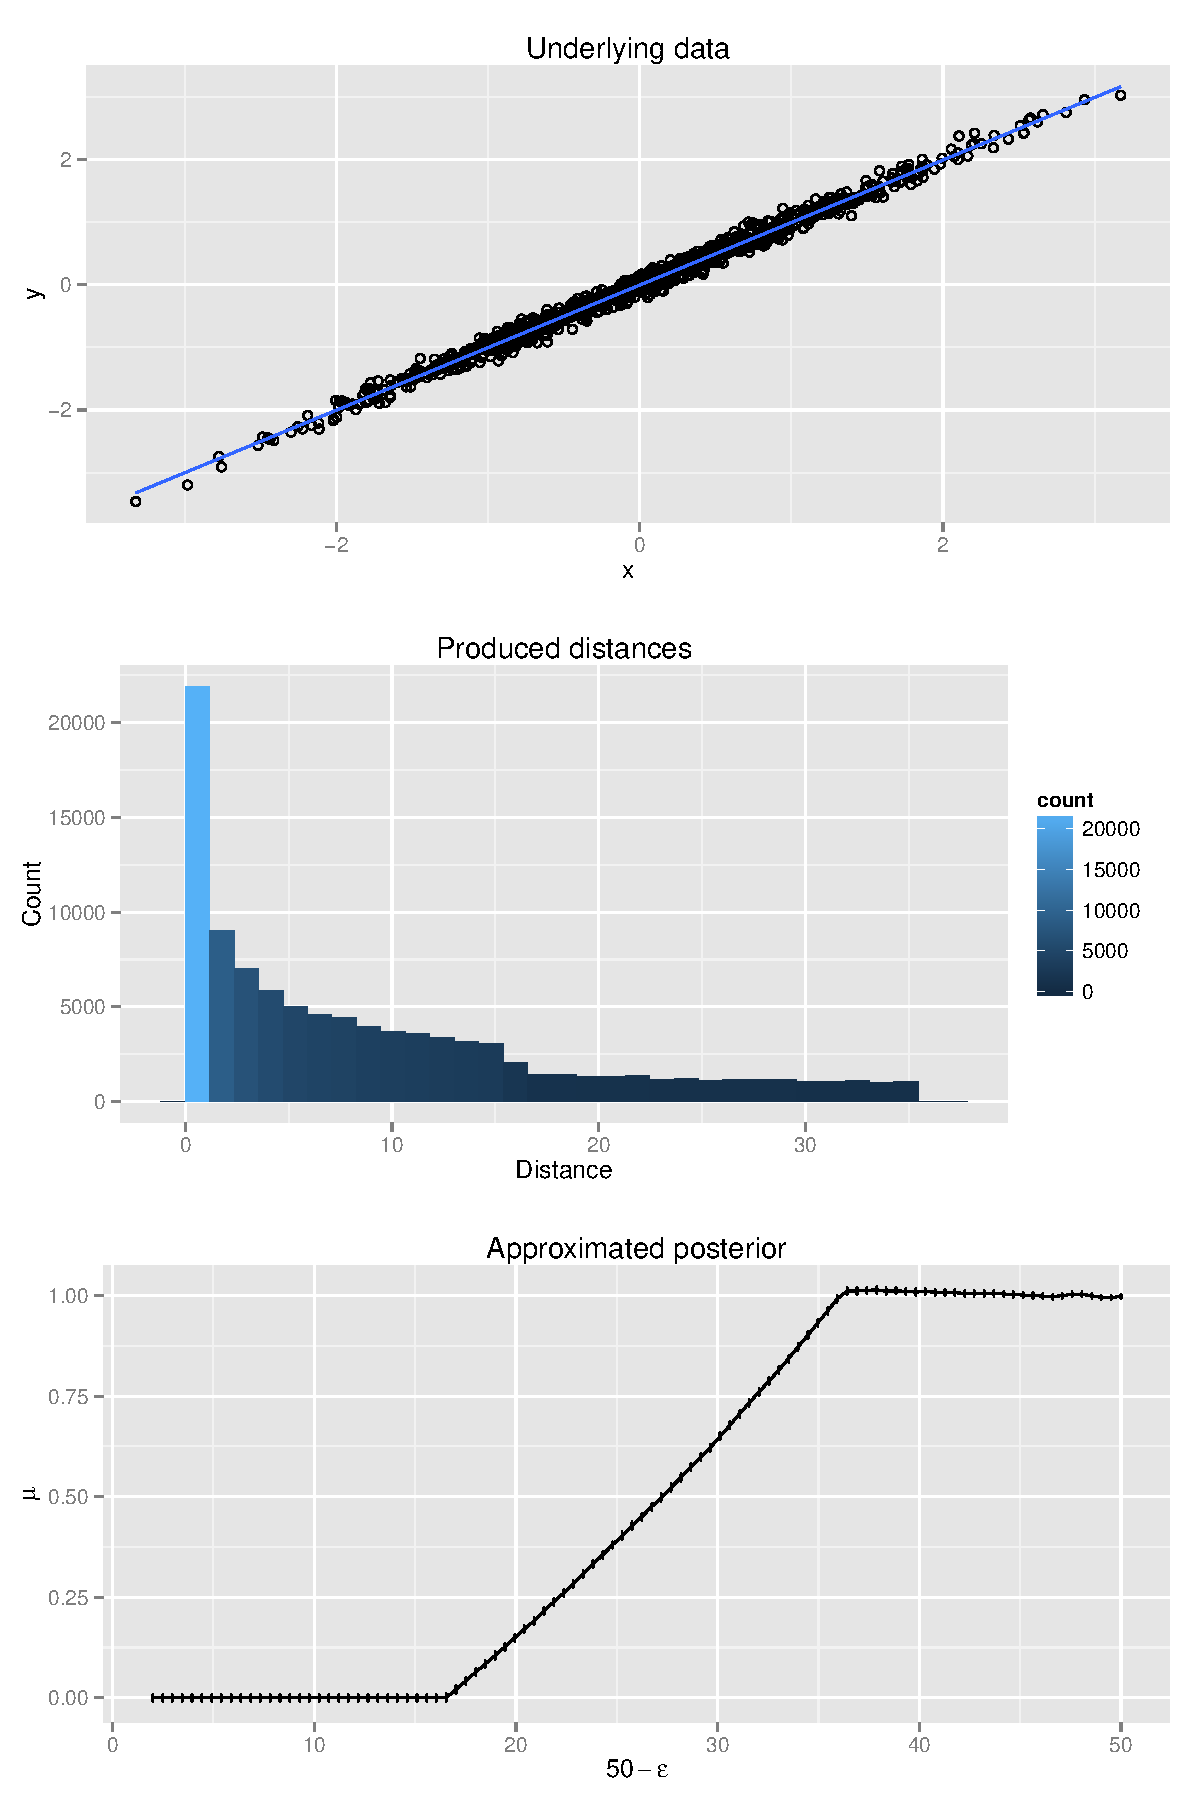
\includegraphics[scale=0.7]{figs/linexample.pdf}
\end{figure}
%END OF ABC EXAMPLE

%%%%%%%%%%%%%%%%%%%%%%%%%%%%%%%%%%%%%%%%%%%%%%%%%%%%%%%%%%%%%%%%%%%%%%%%%%%%%%%%%%%%%%%%%%%%%%%%%%%
%Definition and description of TTB-ABC
%%%%%%%%%%%%%%%%%%%%%%%%%%%%%%%%%%%%%%%%%%%%%%%%%%%%%%%%%%%%%%%%%%%%%%%%%%%%%%%%%%%%%%%%%%%%%%%%%%%

\section{A model to grow heuristic strategies}
Let us now define a model to learn non-compensatory decision strategies from smaller building blocks directly. Given that every heuristic is made up of a search, stopping, and a decision rule, we want to find a model that can result into a similar tree structure as TTB, but which learns the structure of the tree automatically over time. The nodes of such a tree can be seen as small building blocks of the heuristic.  The way these nodes are assembled at the end, then corresponds to the search rule. The implied depth of the tree can be seen as representing the stopping rule which is reached as soon as a node makes a decision. Finally, the decision at a decisive node represents the overall decision rule. The way TTB-ABC learns and makes predictions is sketched out in Algorithm~\ref{alg:ttbabc}.\\

%ALGORITHM
\FloatBarrier
\begin{algorithm}
\caption{TTB-ABC}
\label{alg:ttbabc}
\input{algs/ttbabc.alg}
\end{algorithm}
\FloatBarrier
%END OF ALGORITHM

The function \texttt{ttbabclearn} defines the model's learning process. It starts out with a Beta-prior that induces a likelihood for each cue to be successful. It then samples probabilities from the prior for each cue. These probabilities are then used to generate a proposal tree. The cues for the proposal tree are sampled without replacement and in proportion to the sampled p-values from the prior before. As these betas will be updated based on a cue's success, this means that cues which are more likely to be successful are sampled at the top of the proposal tree with a higher probability than cues that have not been very successful. The built proposal tree is then used and applied to a randomly sampled subset of the whole data. The size of the randomly sampled subset depends on the parameter $\rho$, for which $0<\rho\leq1$, which means that the subset can be anything from one observation to the full data set. The proposed tree is then used to make predictions within the subset and these predictions are compared with the actual outcomes. If more than $\epsilon$ of the predictions turn out to be correct, then the tree is accepted and the involved cues of that tree get updated by adding one success to their posterior beta-binomial-distribution. If too many classifications turn out to be wrong, then the proposal tree is rejected and no update happens. This whole process repeats until $\eta$ successful proposals have been generated and the function returns the posterior beta-binomial-distribution of all cues.

The way this function learns is similar to the linear example described before. The generating model is the implied distribution over cue orders, based on the beta-binomial distribution. The used statistic is the performance in the sub-sample, it is a statistic as it does not use the whole sample, but rather approximates the performance in the whole set based on the sampled set. The way this algorithm updates cues can also be described as a Polya urn sampling scheme, where balls are put into an urn and successful (chosen) balls get reinforced over time. On a more descriptive level, TTB-ABC starts out with a prior over all possible cue orders, which is defined by the current probability of the cues to be chosen. It then generates proposal trees, and checks how well these trees perform within a subset of the data, a current stream of mental simulations, and sanity checks these proposals. It then reinforces successful combinations by a Bayesian reinforcement learning algorithms \citep{poupart2010bayesian} built on Approximate Bayesian Computation. In this way, TTB-ABC starts out with small building blocks (the cues) and puts them together and --over time-- heuristic structures emerge. Notice that TTB is only one possible sub-structure of TTB-ABC. Many other possibly even more greedy strategies can be built. One example of such a strategy is one where one cue takes up more and more of the overall importance and thus almost always gets used on its own.

The function \texttt{ttbabcpredict} takes in as an argument the posterior of the beta-binomial distribution constructed by \texttt{ttbabclearn} and a parameter $n_{aggregate}$.  The posterior is then used again to generate a proposal tree in dependency of how well the cues performed in the training period, and this tree is used to generate predictions for the test set. This procedure is repeated  $n_{aggregate}$ times and the mode of all predictions is used as the final prediction.

Taken together, these two function constitute a first approach to how a cue order can be learned from the very beginning and how a heuristic can emerge by combining smaller building blocks, nodes of trees, and then mentally simulating the success of proposals which generates a process, that --over time-- is able to find and utilize simple trees within the complex forest of all possible trees.  %This is to mention the title in the text, just as they do it in Hollywood...

%this section need a lot more argumentative power, but I don't know how to sell it properly...

%%%%%%%%%%%%%%%%%%%%%%%%%%%%%%%%%%%%%%%%%%%%%%%%%%%%%%%%%%%%%%%%%%%%%%%%%%%%%%%%%%%%%%%%%%%%%%%%%%%
%PERFORMANCE WHEN TTB HAS GENERATED DATA SET
%%%%%%%%%%%%%%%%%%%%%%%%%%%%%%%%%%%%%%%%%%%%%%%%%%%%%%%%%%%%%%%%%%%%%%%%%%%%%%%%%%%%%%%%%%%%%%%%%%%

\section{Recovery performance}
A first sanity check is to see if TTB-ABC can recover the true underlying model from a data set that has been solely produced by TTB. Given the assumption that  TTB is just one subset of all possible models captured by  TTB-ABC, it should be obvious that TTB-ABC can recover TTB from a simulated data set. Thus, 5 independent variables $\mathbf{X=(x_1,x_2, \dots, x_4)}^\top$ were created by using a trinomial distribution, where each vector represents the results of pairwise comparisons of two hypothetical objects (for example, cities). The probability for the first object to win (1) was fixed to be the same as for the second object to win (-1), which was half of that of a draw (0). Therefore, $p(x_i=D)=p(x_i=W \lor L)=\frac{1}{2}$ which means that a draw was set up to be as likely as a decision at each node and $p(x_i=W)=0.25$. The final outcome, which was binary with $y=(0,1)$, was produced by the underlying TTB-model shown in Figure~\ref{fig:ttbtruth} below. The decision strategy generating this data set is exactly the same as normal TTB, i.e. it could be seen as a comparison between two different cities just like in the example above, where a win means that city A has something that city B has not (for example, an airport) and an outcome of $y=1$ means that city A is bigger than city B. However, one of the provided cues is uninformative as it was not included in the underlying model. Therefore, we expect our TTB-ABC model to recover a tree structure that looks like the one shown in Figure~\ref{fig:ttbtruth}.

%BEGIN OF TIKS PICTURE
\FloatBarrier
\begin{figure}
\caption{Underlying TTB-model. Only cues $C_1, C_2,C_3$ are important.}
\label{fig:ttbtruth}
\begin{center}
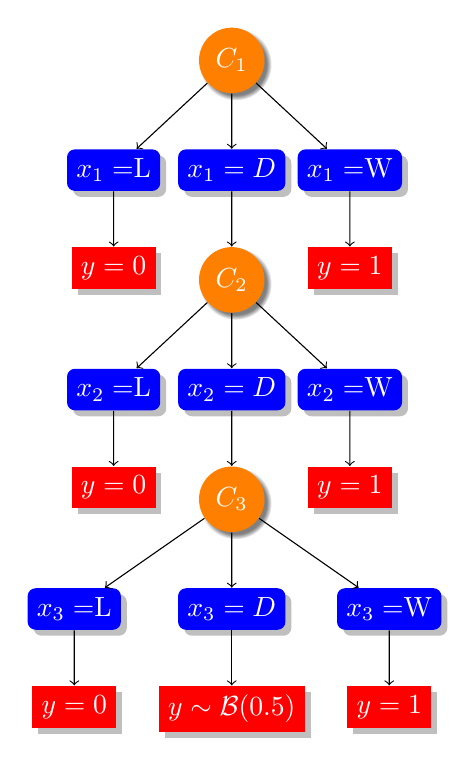
\begin{tikzpicture}[
    fact/.style={rectangle, draw=none, rounded corners=1mm, fill=blue, drop shadow,
        text centered, anchor=north, text=white},
    state/.style={circle, draw=none, fill=orange, circular drop shadow,
        text centered, anchor=north, text=white},
    leaf/.style={rectangle, draw=none, fill=red, drop shadow,
        text centered, anchor=north, text=white},
    level distance=0.7cm, growth parent anchor=south
]
\node (State00) [state] {$C_1$} [->]
child{
        node (Fact01) [fact] {$x_1=$L}
child{
                            node (State03) [leaf] {$y=0$}
                        }
        }
    child{
        node (Fact01) [fact] {$x_1=D$}
        child{
            node (State01) [state] {$C_2$}
           child{
        node (Fact04) [fact] {$x_2=$L}
child{
                            node (State05) [leaf] {$y=0$}
                        }
        } 
           child{
                node (Fact02) [fact] {$x_2=D$}
                child{ [sibling distance=2cm]
                    node (State02) [state] {$C_{3}$}
child{
        node (Fact31) [fact] {$x_3=$L}
child{
                            node (State33) [leaf] {$y=0$}
                        }
        }
                    child{[sibling distance=9cm]
                        node (Fact03) [fact] {$x_3=D$}
                        child{
                            node (leafguess) [leaf] {$y\sim \mathcal{B}(0.5)$}
                        }
                    }
child{
        node (Fact99) [fact] {$x_3=$W}
child{
                            node (State99) [leaf] {$y=1$}
                        }
        }
}}
child{
        node (Fact100) [fact] {$x_2=$W}
child{
                            node (State100) [leaf] {$y=1$}
                        }
        }
}}
child{
        node (Fact01) [fact] {$x_1=$W}
child{
                            node (State03) [leaf] {$y=1$}
                        }
        }

                    
;
        
\end{tikzpicture}

\end{center}
\end{figure}
\FloatBarrier
%END OF TIKS PICTURE

A data set of size $n=1000$ was created and the algorithm was run until 100 proposed trees were accepted. Figure~\ref{ttbrecover} shows the trace plots of the cue importance and the cue weights over time. The traces were calculated by dividing the p-value of each beta posterior mean by the total sum of values over all cues. This then equals the probability of a cue to be chosen. It can be seen that --even after a few accepted proposals-- the mode tree (that is the most likely tree) is the same as the one generating the data. Shortly after the begin of the simulation, the cue order grows to the correct ranking, and the unimportant cue is chosen less frequently, exactly as expected given the underlying structure.

%BEGIN OF CUE IMPORTANCE TRACE PLOT
\begin{figure}[htb!]
  \caption{Trace plots of recovery simulation}
\label{ttbrecover}
  \centering
    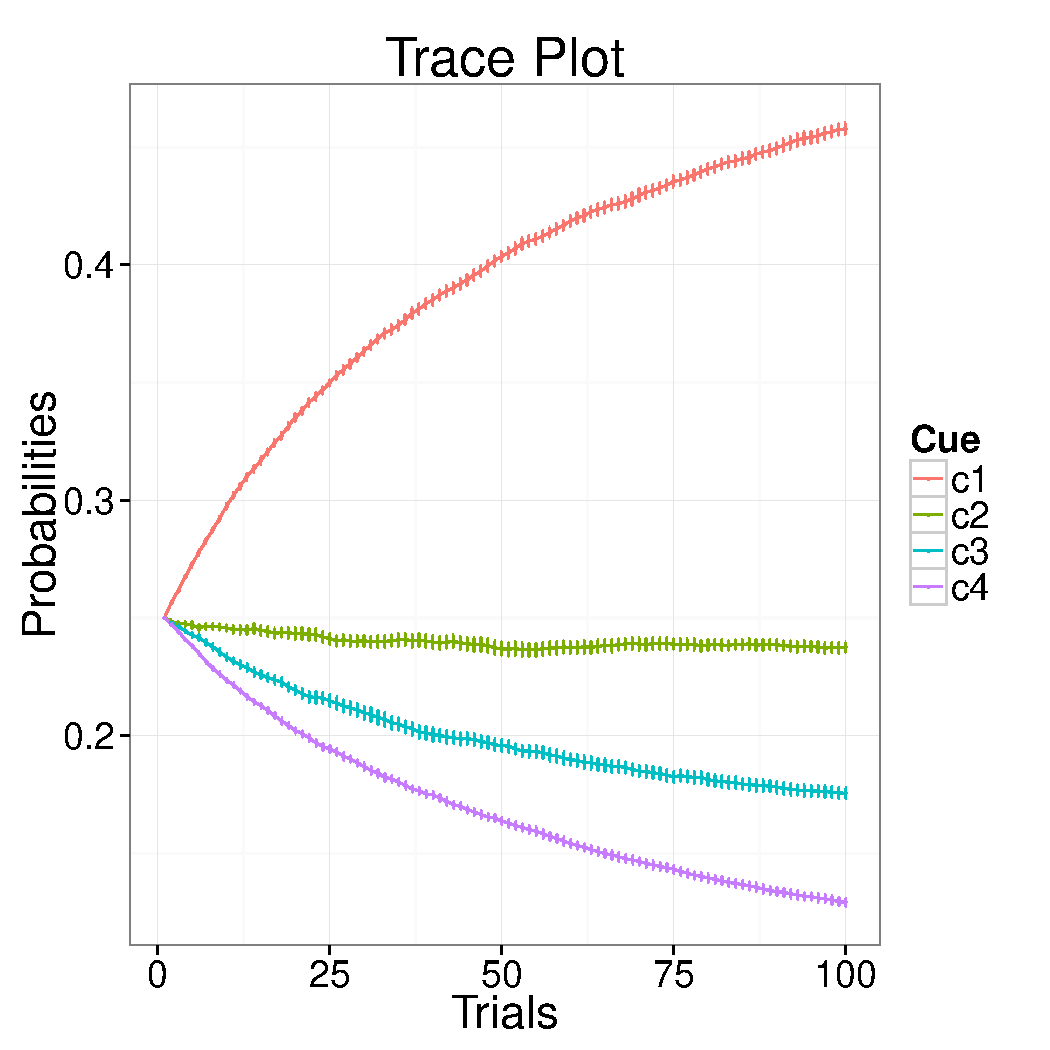
\includegraphics[scale=0.5]{figs/ttbrecovertrace.pdf}
\end{figure}
%END OF CUE IMPORTANCE TRACE PLOT

A plot of the density over all possible trees is shown in Figure~ref{fig:treedense}. It can be seen that the density for the right tree (C1,C2,C3,C4) becomes more and more likely over time.

%I'm gonna redo this plot soon with better convergence and smaller alpha. also saving it as .png might save some kbs...
%BEGIN OF TREE DENSITY PLOT
\begin{figure}[htb!]
  \caption{Density over trees per sampling step}
\label{fig:treedense}
  \centering
    \includegraphics[scale=0.5]{figs/treedensity.pdf}
\end{figure}
%END OF TREE DENSITY PLOT

%%%%%%%%%%%%%%%%%%%%%%%%%%%%%%%%%%%%%%%%%%%%%%%%%%%%%%%%%%%%%%%%%%%%%%%%%%%%%%%%%%%%%%%%%%%%%%%%%%%
%INFERENCE AND PREDICTIONS IN CITY SIZE DATA SET
%%%%%%%%%%%%%%%%%%%%%%%%%%%%%%%%%%%%%%%%%%%%%%%%%%%%%%%%%%%%%%%%%%%%%%%%%%%%%%%%%%%%%%%%%%%%%%%%%%%

\section{Inference for real data}

%In this section, we could actually use more data sets
%Also, we could compare inference to the actual underlying tree
%Compare different cue validity functions?
Another check is whether or not TTB-ABC generates sensible and interpretable inferences in a real data set. Thus, we applied our algorithm to the classic city size data set in order to see how the trace plot looks like for this data. The city size data set has been frequently used in the past and contains 9 different binary variables that all can be used to decide which of two cities is bigger \citep{chater2003fast, gigerenzer2009homo}. Figure~\ref{fig:citytrace} shows the trace plots for the city size simulation over 100 accepted proposal trees. Again, the output looks sensible, finding that having a university, an exposition site, and a major league soccer team are the three most important cues.

%BEGIN OF CITY CUE IMPORTANCE TRACE PLOT
\begin{figure}[htb!]
  \caption{Trace plots of city size data estimation.}
\label{fig:citytrace}
  \centering
    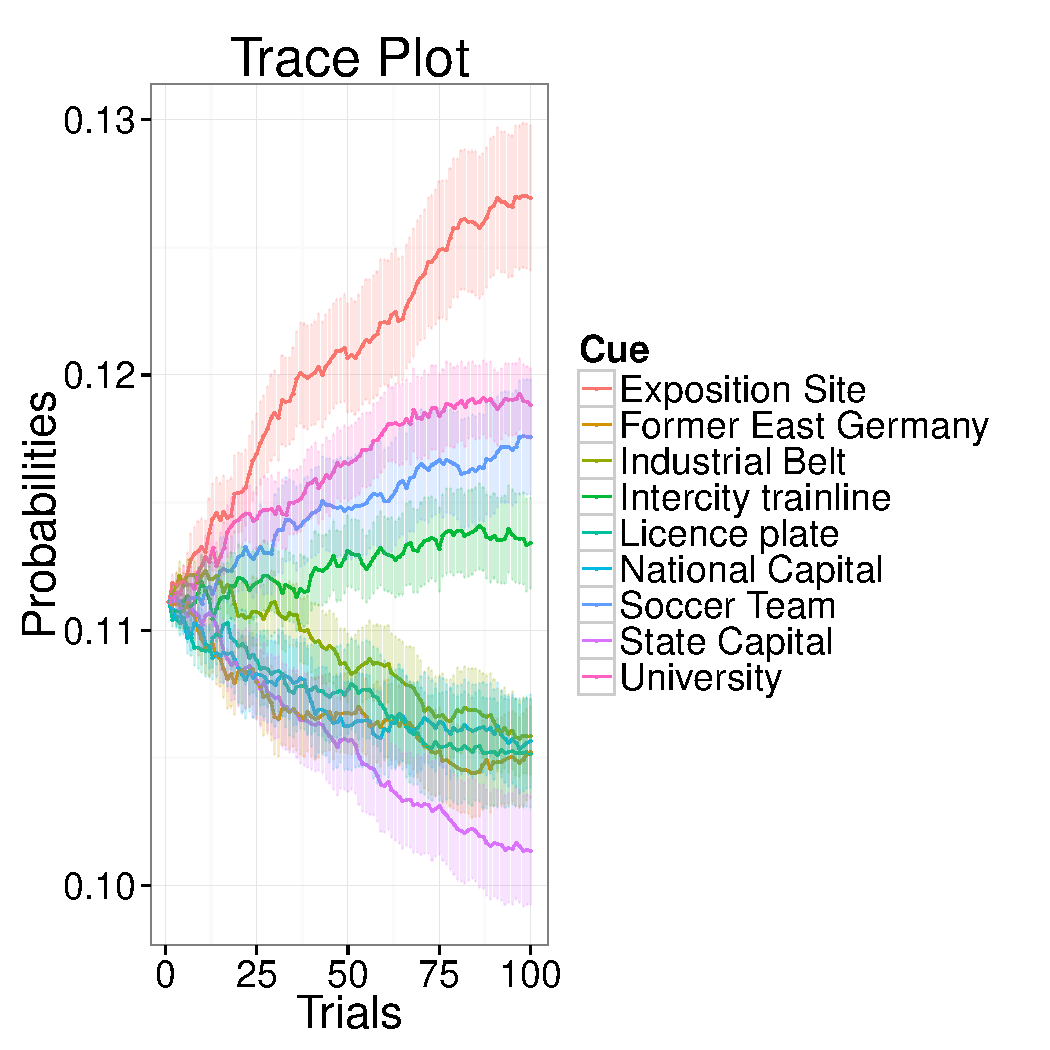
\includegraphics[scale=0.5]{figs/citytrace.pdf}
\end{figure}
%END OF CITY CUE IMPORTANCE TRACE PLOT

Notice that contrary to the classic estimation of TTB, the capital city cue turned out to decrease in probability over time instead of being the most important cue. This is due to the fact that Berlin is the only city in the whole data set that is a capital city and therefore this cue could not be applied very often, a finding that has been coped with in the literature before \citep{broder2012quest}.

%%PREDICTIONS
\section{Predictive comparison}
Another important benchmark is how well TTB-ABC can predict different outcomes. Therefore, we sought out to compare TTB-ABC's predictive performance within three different data sets: the city size data, professors' salary, and homelessness in the US. We let three different TTB models learn within a learning set and classify new items within a test set.  TTB-ABC was fitted by using the algorithm described above. Standard TTB was fitted by calculating the cue validity in the way originally proposed:

\begin{align}
v=\frac{\mathbbm{1}_{x_i=y_i}}{\sum_i^n{\mathbbm{1}_{x_i\neq0}}}
\end{align}
which basically just sums up how often a cue can be used to make a successful predictions, given that it can be used at all. TTB-Updated is trying to adjust for this problem \cite{newell2004search} and corrects the cue validity by the discrimination rate, that is how often a cue can actually be applied.

\begin{align}
d&=\frac{\sum_{i=1}^{n}{\mathbbm{1}_{x_i \neq y_i}}}{n}\\
v_{\text{updated}}&=v \times d+0.5\times(1-d)
\end{align}

In order to see which of the two models performs best for different sizes, test sets were created to be of the size $s=\{10\%,20\%,\dots,90\%\}$ of the total data set (before the comparisons were generated). The learning set always contained the remaining data points that were not used in the test set. For every size, 50 randomly generated repetitions were run and the mean performance was tracked.  

Additionally, for each data set, we calculated the best possible cue order for the whole data set by a brute force algorithm directly. Brute force means that all possible cue combinations were generated and the one that overall lead to the lowest classification error was taken to be the best order. This order could then be compared to the order determined by each model and also tracked for different set sizes over the 50 trials. The distance to the best underlying cue order was calculated by using the discounted cumulative gain as shown in Equation~\ref{eq:dcg} \citep{netharecognizing}.

\begin{align}
\label{eq:dcg}
DCG_l=\sum_{i=1}^{l}\frac{Q_i}{\log_2(i+1)}
\end{align}

The resulting sum is then divided by the best possible order, which was determined by the brute force algorithm and again tracked overall.
Results are shown in Figure~\ref{fig:performance}. It can be seen that TTB-ABC outperforms standard TTB across the whole range. This finding is even more surprising given that TTB has consistently been found to outperform many other models within this data set.

%BEGIN OF PREDICTIVE PERFORMANCE PLOT
\begin{figure}[htb!]
  \caption{Performance of different models in dependency of training size}
\label{fig:performance}
  \centering
    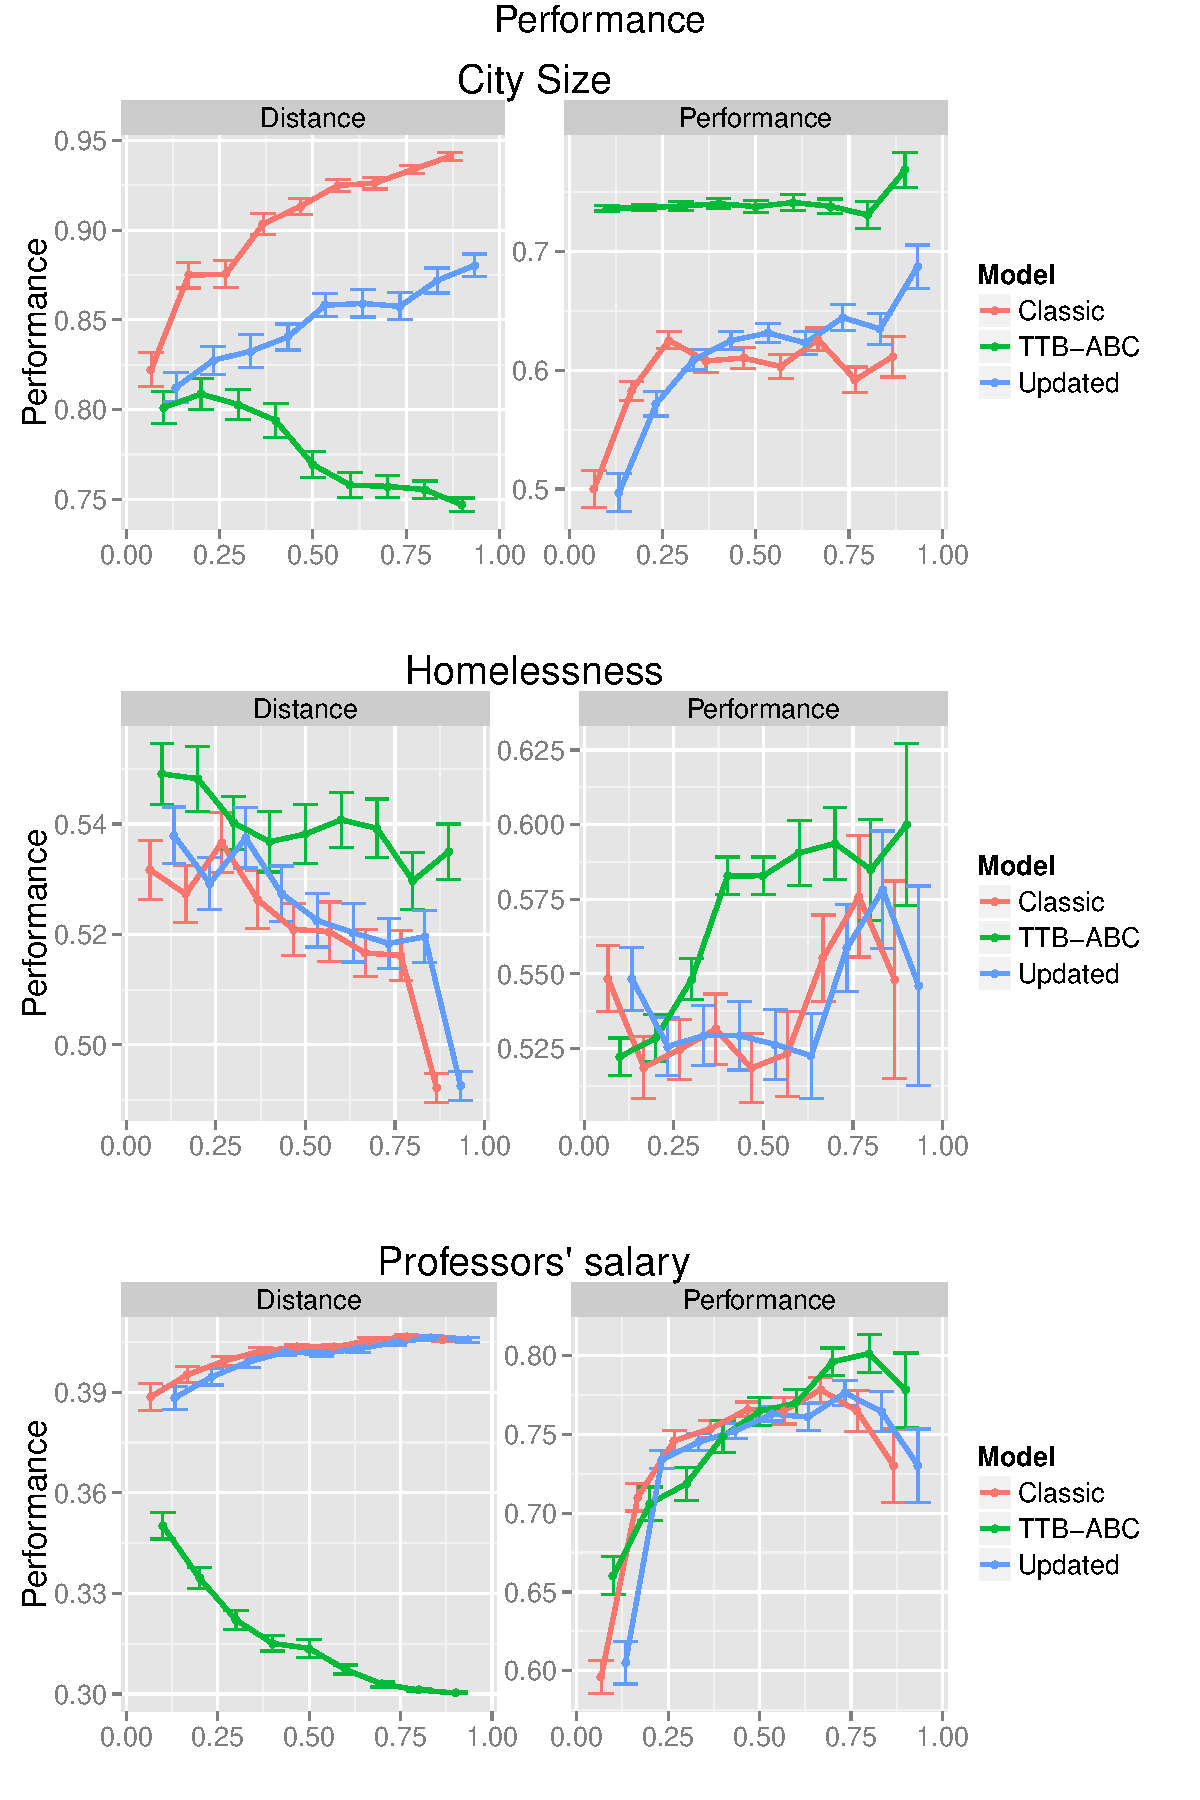
\includegraphics[scale=0.7]{figs/performance.pdf}
\end{figure}
%END OF PREDICTIVE PERFORMANCE PLOT

It can be seen that TTB-ABC performs better than the other two approaches across all different data sets. However, on average, TTB-ABC tends to decrease in its ability to find the best possible cue order. This is due to the fact that only the mode cue order, that is the most likely a posteriori order, has been used for this calculation. Moreover, the number of samples that TTB-ABC samples naturally get smaller as the learning set gets bigger. In general though, TTB-ABC performs better than the other two approaches while generating simple distributions over cue orders at the same time.

%%%%%%%%%%%%%%%%%%%%%%%%%%%%%%%%%%%%%%%%%%%%%%%%%%%%%%%%%%%%%%%%%%%%%%%%%%%%%%%%%%%%%%%%%%%%%%%%%%%
%TRADING OFF COMPLEXITY AND PERFORMANCE
%%%%%%%%%%%%%%%%%%%%%%%%%%%%%%%%%%%%%%%%%%%%%%%%%%%%%%%%%%%%%%%%%%%%%%%%%%%%%%%%%%%%%%%%%%%%%%%%%%%

\section{Trading off performance and computation time}
Another benefit of our TTB-ABC model is that performance and computational time can be traded-off against each other explicitly. As the $\epsilon$-parameter defines the proportions of predictions that have to be correct in order for a proposal tree to be accepted, increasing this parameter will lead to more proposal trees being rejected. This in turn will lead to a longer computation time as more proposals have to be created overall. However, better proposals also mean better performance as the proposals have a better quality. The $\eta$-parameter in turn determines the number of accepted proposed trees. Thus, more accepted trees means more proposals needed, means longer computation time, which in again will lead to better performance. The same holds true for the proportion of sampled data points $\rho$. The higher the proportion of the sampled data set, the better the proposed trees have to be, and the longer it takes to find good trees. 

Using \texttt{ttbabclearn}, we can model these parameters explicitly to find out how they influence performance and computation time (here used as a proxy variable for complexity). Therefore, we created all 81 possible combinations of $\epsilon=\{0.1,0.2,\dots,0.9\}$ and $\rho=\{0.1,0.2,\dots,0.9\}$ and applied the resulting model to the scenario in which TTB had generated the data as in the first recovery task above. The resulting models were applied to this data set with $\eta=\{1,10,50,100\}$ simulations. We used the R-package \texttt{microbenchmark} to track the the time it took to learn within the different sets, averaged over 100 trials. The results of the overall computation time are shown in Figure~\ref{fig:timetradeoff} below.
%BEGIN OF PERFOMANCE TRADE-OFF PLOT
\begin{figure}[htb!]
  \caption{Assessed computational time of different $\epsilon$-$\rho$-combinations for $\eta=\{1,10,50,100\}$ samples.}
\label{fig:timetradeoff}
  \centering
    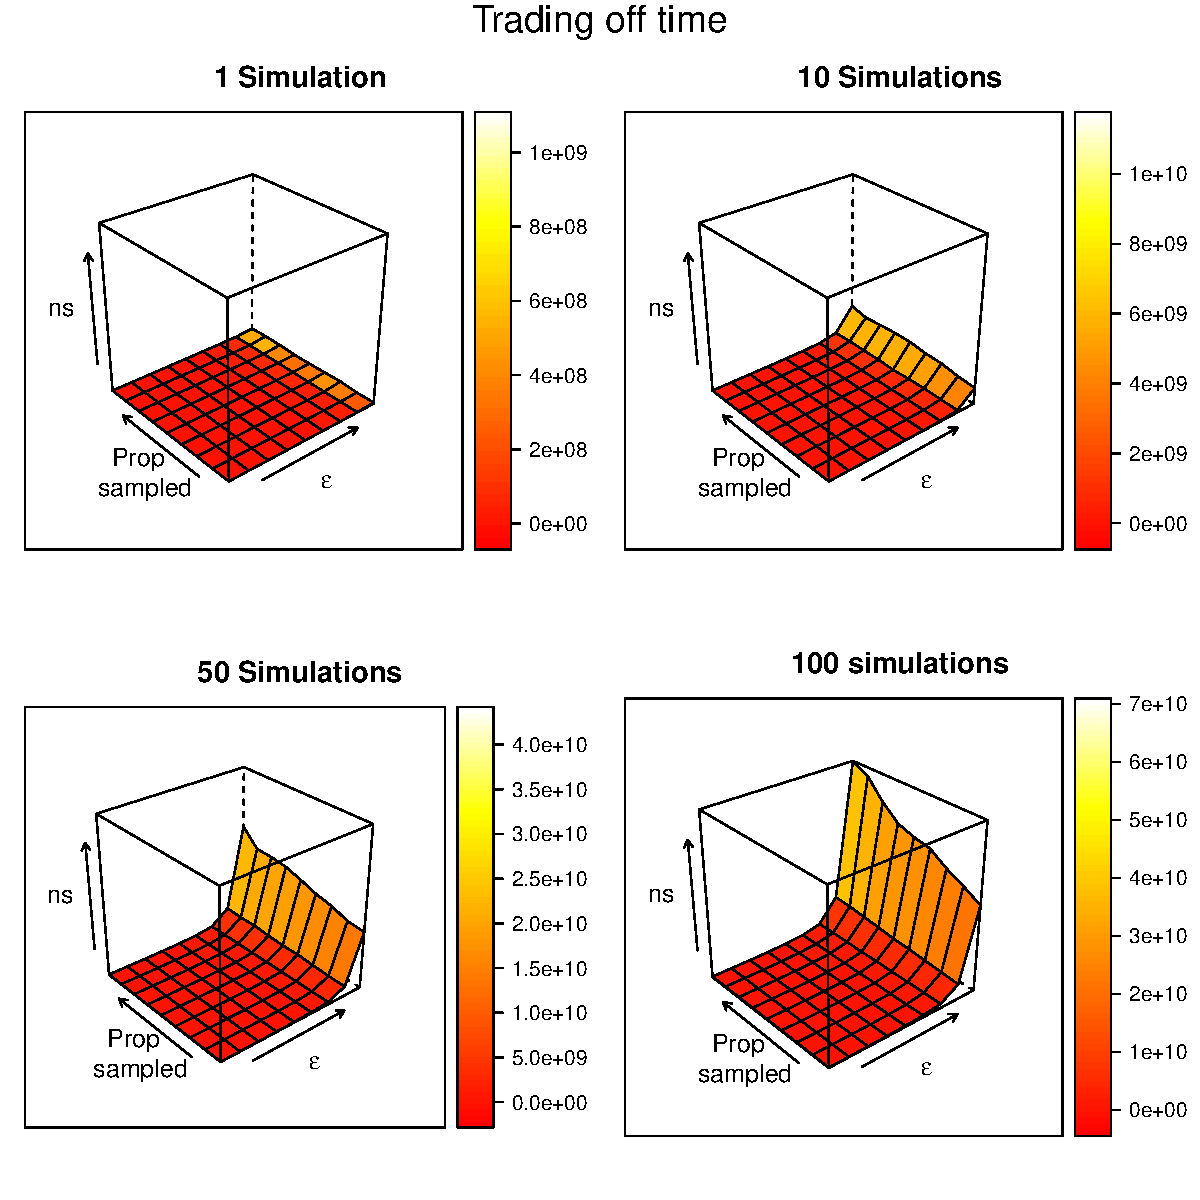
\includegraphics[scale=0.6]{figs/timetradeoff.pdf}
\end{figure}
%END OF TIME TRADE-OFF PLOT
We can see that for low $\eta$s, the computational time does not differ much for high and low $\epsilon$s and $\rho$s. However, for many number of simulations, the computation time seems to increase exponentially, if the proportion of samples as well as the quality of the to be accepted models increases.

For the performance of the resulting models, we averaged the models' predictions over the whole set over 30 trials and calculated the mean proportion of correct predictions over the whole set. Results are shown in Figure~\ref{fig:performancetradeoff}.
%BEGIN OF PERFOMANCE TRADE-OFF PLOT
\begin{figure}[htb!]
  \caption{Assessed performance of different $\epsilon$-$\rho$-combinations for $\eta=\{1,10,50,100\}$ samples.}
\label{fig:performancetradeoff}
  \centering
    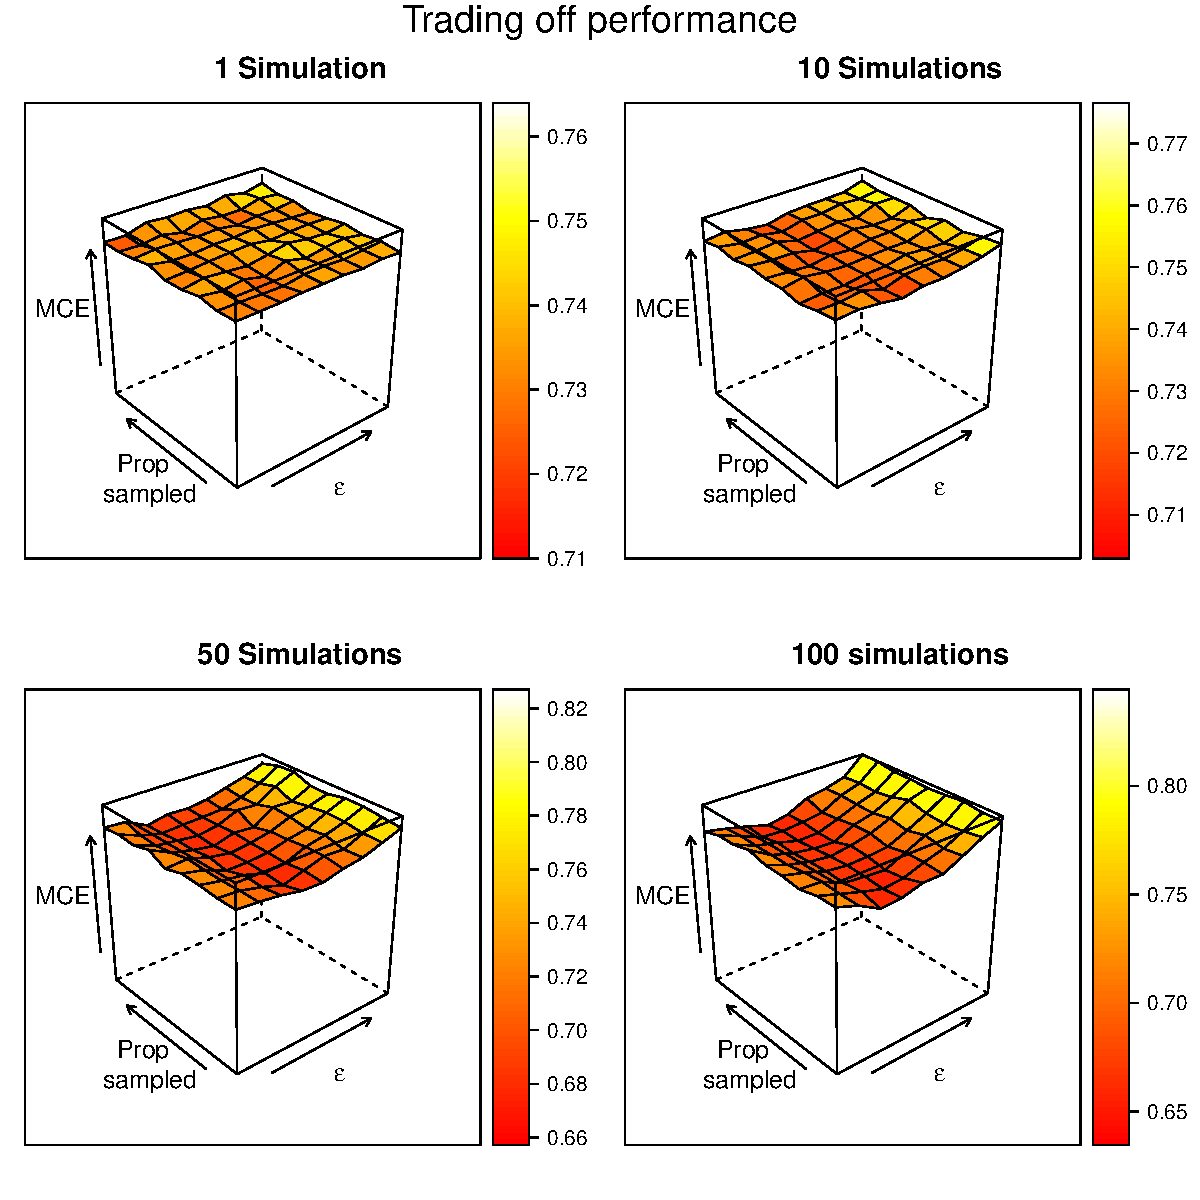
\includegraphics[scale=0.6]{figs/performancetradeoff.pdf}
\end{figure}
%END OF PERFOMANCE TRADE-OFF PLOT

We can see that, especially for high number of samples $\eta$, tuning the $\epsilon$ and $\rho$-parameters can increase performance by up to 20\%, whereas for lower sample numbers the configuration matters less.

Taking these two results together, we see that there seems to be a clear trade-off between time and performance as time increases exponentially, but performance increases not as much as time. The performance gained per time spent therefore increases with the number of samples. Using TTB-ABC we can model this trade-off explicitly by changing the different parameters and actually test the performance-accuracy trade-off, a crucial assumption of heuristic theories of decision making, directly.

%%%%%%%%%%%%%%%%%%%%%%%%%%%%%%%%%%%%%%%%%%%%%%%%%%%%%%%%%%%%%%%%%%%%%%%%%%%%%%%%%%%%%%%%%%%%%%%%%%%
%DISCUSSION AND CONCLUSION
%%%%%%%%%%%%%%%%%%%%%%%%%%%%%%%%%%%%%%%%%%%%%%%%%%%%%%%%%%%%%%%%%%%%%%%%%%%%%%%%%%%%%%%%%%%%%%%%%%%

\section{Discussion \& Conclusion}
We have introduced TTB-ABC, a model that can grow heuristic decision trees via Approximate Bayesian Computation. Using an approximately Bayesian learning scheme, this algorithm can learn heuristic decision strategies over time and constitutes as a first proposal of how a tool from the heuristic toolbox can emerge from smaller building blocks.

We have shown that TTB-ABC can recover original TTB in a simple simulated data set and leads to sensitive estimates of expected cue depth, cue orders, and cue weights within the frequently used city size data set. In a predictive performance task, TTB-ABC outperformed TTB across the board, even though it can lead to more simple inferences at the same time. Lastly, TTB-ABC can be used to model the time-accuracy trade-off directly by adjusting its input parameters. Doing so, we have found that there are scenarios where increased computation time diminishes in returns of predictive accuracy.

TTB-ABC constitutes as a first proof of concept that a heuristic can emerge from smaller building blocks over time and we expect it to be further developed as well as applied to human experimental data soon. 

Other ways of letting strategies emerge over time such as inductive programming \citep{muggleton1994bayesian}, evolutionary (symbolic) regression \citep{dechter2013bootstrap}, as well as the composition of smaller sub-units via greedy search algorithms \citep{duvenaud2013structure} could also be defined and tested in future studies.

In the long term, a valid goal for heuristic theories of decision making seems to be defining how many different heuristic models, that is not only tree-like structures, can emerge from smaller compositional building blocks, thereby defining a grammar of rules within a heuristic toolbox.

%%%%%%%%%%%%%%%%%%%%%%%%%%%%%%%%%%%%%%%%%%%%%%%%%%%%%%%%%%%%%%%%%%%%%%%%%%%%%%%%%%%%%%%%%%%%%%%%%%%
%BIBLIOGRAPHY
%%%%%%%%%%%%%%%%%%%%%%%%%%%%%%%%%%%%%%%%%%%%%%%%%%%%%%%%%%%%%%%%%%%%%%%%%%%%%%%%%%%%%%%%%%%%%%%%%%%
\bibliographystyle{apa-good}
\bibliography{Mybibo}
\end{document}
%END OF DOCUMENT